\documentclass{beamer}

\usepackage{multicol}

\usetheme{Warsaw}

\title{Uppaal. The Model Checker.}
\author{Patryk Kiepas}
\date{\today}

\begin{document}
%-------------------------------------------------------------------------
\begin{frame}
	\titlepage
\end{frame}

%-------------------------------------------------------------------------	
\section*{Outline}
\begin{frame}
	\tableofcontents
\end{frame}

%%%%%%%%%%%%%%%%%%%%%%%%%%%%%%%%%%%%%%%%%%%%%%%%%%%%%%%%%%%%%%%%%%%%%%%%%%
\section{Intro}
%%%%%%%%%%%%%%%%%%%%%%%%%%%%%%%%%%%%%%%%%%%%%%%%%%%%%%%%%%%%%%%%%%%%%%%%%%
\subsection{Quick look}
%-------------------------------------------------------------------------
\begin{frame}
	Uppaal is a model checker for real-time systems. What we can with it?
	
	\begin{enumerate}
		\item Modeling
		\item Simulation
		\item Verification
	\end{enumerate}
	
	Internal representation of model consists of:
	
	\begin{itemize}
		\item Network of timed automata
		\item Extended with data types
	\end{itemize}

\end{frame}


\subsection{History}
%-------------------------------------------------------------------------
\begin{frame}
	Uppaal was started by Uppsala University, Sweden and Aalborg University, Denmark.
	
	Timeline of development:
	\begin{itemize}
		\item 1995 - project started
		\item 1999 - first beta
		\item 1999/2000 - first stable release (v 3.0.X)
		\item September 27, 2010 - latest stable release (v 4.0.13)
		\item July 1, 2014 - preview release (v 4.1.19)
	\end{itemize}
	
	Versions: Windows, Mac, Linux, 32/64 bits
	
	Available licenses:
	\begin{itemize}
		\item Academic use (more info: \href{http://www.uppaal.org/}{http://www.uppaal.org/})
		\item Commercial use (more info: \href{http://www.uppaal.com/}{http://www.uppaal.com/})
	\end{itemize}
\end{frame}


%%%%%%%%%%%%%%%%%%%%%%%%%%%%%%%%%%%%%%%%%%%%%%%%%%%%%%%%%%%%%%%%%%%%%%%%%%	
\section{The tool}
%%%%%%%%%%%%%%%%%%%%%%%%%%%%%%%%%%%%%%%%%%%%%%%%%%%%%%%%%%%%%%%%%%%%%%%%%%
\begin{frame}{Uppaal GUI - Main parts}
\vspace{-10mm}
\begin{columns}
	\begin{column}{0.8\textwidth}
		\begin{figure}[H]
			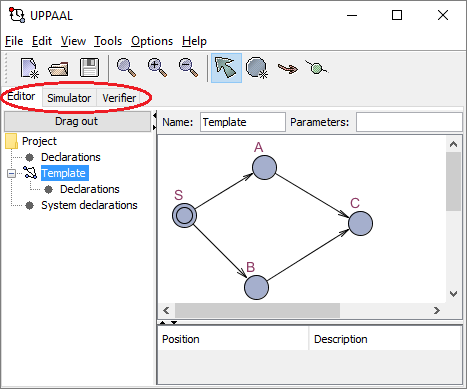
\includegraphics[scale=0.7]{img/uppaal_gui_small_editor.png}
		\end{figure}
	\end{column}
	
	\begin{column}{0.3\textwidth}
		\begin{itemize}
			\item System editor
			\item Simulator
			\item Verifier
		\end{itemize}
	\end{column}
\end{columns}		
\end{frame}

\begin{frame}{Uppaal GUI - Editor control}
	\vspace{-10mm}
	\begin{columns}
		\begin{column}{0.8\textwidth}
			\begin{figure}[H]
				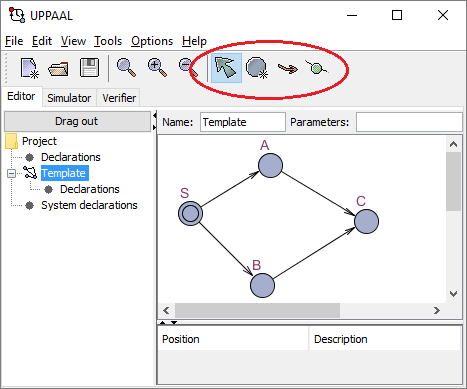
\includegraphics[scale=0.7]{img/uppaal_gui_small_editor_control.png}
			\end{figure}
		\end{column}
		
		\begin{column}{0.3\textwidth}
			\begin{itemize}
				\item Name: Template (defualt)
				\item Select
				\item Add location
				\item Add edge
				\item Add nail
			\end{itemize}
		\end{column}
	\end{columns}		
\end{frame}

\begin{frame}{Uppaal GUI - Simulation control}
	\vspace{-5mm}
	\begin{columns}
		\begin{column}{0.8\textwidth}
			\begin{figure}[H]
				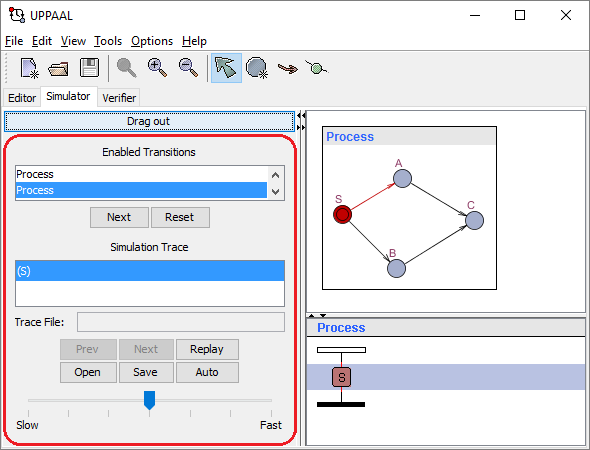
\includegraphics[scale=0.55]{img/uppaal_gui_small_simulation.png}
			\end{figure}
		\end{column}
		
		\begin{column}{0.35\textwidth}
			\begin{itemize}
				\item Select transition
				\item Track simulation
				\item Control (Prev/Next/Auto)
				\item Visualization
			\end{itemize}
		\end{column}
	\end{columns}		
\end{frame}

\begin{frame}{Uppaal GUI - Verification}
	\vspace{-5mm}
	\begin{columns}
		\begin{column}{0.8\textwidth}
			\begin{figure}[H]
				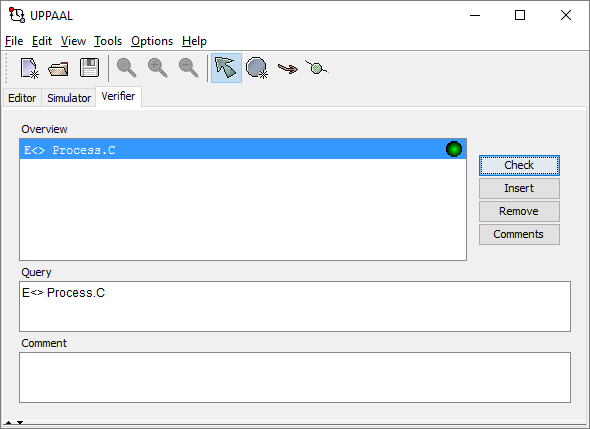
\includegraphics[scale=0.55]{img/uppaal_gui_small_verification.png}
			\end{figure}
		\end{column}
		
		\begin{column}{0.35\textwidth}
			\begin{itemize}
				\item Query editor
				\item Check query
				\item Overview
				\item Save/load
			\end{itemize}
		\end{column}
	\end{columns}		
\end{frame}

%%%%%%%%%%%%%%%%%%%%%%%%%%%%%%%%%%%%%%%%%%%%%%%%%%%%%%%%%%%%%%%%%%%%%%%%%%	
\section{Example}
%%%%%%%%%%%%%%%%%%%%%%%%%%%%%%%%%%%%%%%%%%%%%%%%%%%%%%%%%%%%%%%%%%%%%%%%%%

\end{document}
